\chapter{Desarrollo}

Para la propuesta de arquitectura se consideraron aspectos como: rendimiento, estructura de código, escalabilidad y estabilidad. Otro factor que influyó en la toma de desiciones sobre los componentes a utilizar fue el uso que sector productivo les ha dado.

Resultado de este analisis, se llegó a la conclusión de utilizar Java EE como base de la arquitectura, esto debido a el enfoque empresarial con el que cuenta el Framework, además de adaptarse a librerias y frameworks de terceros para complementar sus funciones.

Una vez definida la tecnología base , el siguiente punto fue definir el tipo de arquitectura que se implementará. Coniderando los estandares e investigaciones actuales, se optó por una arquitectura SOA, pues este modelo ofrece flexibilidad y rendimiento para el desarrollo de sistemas creando módulos independientes que son fáciles de crear y mantener.

Para desarrollar un sistema bajo la arquitectura SOA, se deben separar las capas que lo conformen, para esta se proponen 3 capas: Presentación, Lógica de Negocios y Resursos. Los componenes que integren cada capa se analizarán a detalle en apartados posteriores.

\section{Descripción general de la Arquitectura}
La arquitectura estará separada en 3 capas de manera que se puedan desarrollar servicios web independientes y estos puedan ser consumidos por la capa de presentación, cada capa estará representada por un proyecto java diferente como se muestra en la siguiente figura:

\begin{figure}[H]
  \begin{center}
    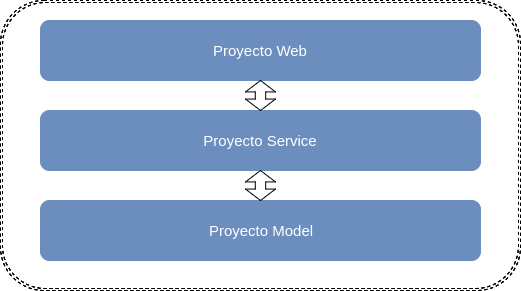
\includegraphics[scale= 0.5]{Propuesta}
  \end{center}
  \caption{Separación por capas}
\end{figure}

El proyecto web funciona como la capa de presentación, el service como la capa de lógica de negocio, y la de model como la capa de recursos. 

A continuación se analizará el funcionamiento interno de capa capa o proyecto así como los componentes que influyen en cada una:

\subsection {Capa de presentación}
La capa de presentación es la encargada de la interacción con el usuario final, esta capa se conecta con la de lógica de negocio para completar los procesos del sistema.
En la arquitectura esta capa está representada por el proyecto "web", cuya estructura se representa en la siguiente figura:

Como se puede observar en la figura anterior, es un proyecto MVC Java Server Faces, esto es una de las ventajas de la arquitectura SOA, cada proyecto puede tener una arquitectura interna sin interferir en las demás capas. 

\subsubsection{Vista}

La vista está conformada por elementos xHTML. El formato es utilizado por JSF para la definición de la estructura de la interfaz de usuario.
Para facilitar el proceso de construcción de interfaz, se utilizan componentes preconstruidos que se incluyen en el framework PrimeFaces.

\subsubsection{Controlador y Modelo}

Una de las caracteristicsa de JSF es la división de elementos html y lógica de negocio mediante clases denominadas ManagedBeans.
Los ManagedBeans son utilizados para dar funcionalidad a los eventos creados en la Vista, en esta arquitectura se utilizarán para conectar este proyecto con la capa de servicio (lógica de negocio).
Un ManagedBean es una simple clase Java, pero con anotaciones especiales que la diferencien. Los metodos de esta clase realizaran peticiones a la capa de servicio, esa capa regresará un resultado en formato JSON, el cual será procesado por la vista para visualiar los datos que el usuario final espera.

\subsection{Capa de Lógica de Negocio}

El proyecto "service" se encarga de la capa de Lógica de Negocio, en esta capa se orquestan los servicios necesarios por el sistema. 
Este proyecto se conecta con la capa de modelo para realizar operaciones CRUD (crear, leer,actualizar, y remover) sobre los modelos establecidos, mediante controladores REST proporcionados por Spring, como el que se muestra a continuación:


\begin{lstlisting}
@RestController
@RequestMapping("/ws")
public class EmpleadoWS {
    @Autowired
    private EmpleadoService empleadoService;
    
    @RequestMapping(method = RequestMethod.GET, value = "/login")
    @ResponseBody
    public Empleado login(
      @RequestParam(value = "usuario")String usuario,
      @RequestParam(value = "contrasena")String contrasena){
        return empleadoService.login(usuario, contrasena);
    }
}
\end{lstlisting}
Una vez que las operaciones solicitadas por la vista se realizan, el ManagedBean envía una respuesta con la informacón solicitada, o algún código de confirmación.

\subsection{Capa de Recursos}
La capa de recursos se encarga del acceso a los modelos o entidades que el sistema manipulará, es por esto que dentro de la aplicacion Java, esta capa se representa con el proyecto "model".

\section{Descripción de componentes por capa}

A continuación se describirá a detalle los componentes utilizados en cada capa de la arquitectura.

\subsection{Capa de Presentación}

\begin{figure}[H]
  \begin{center}
    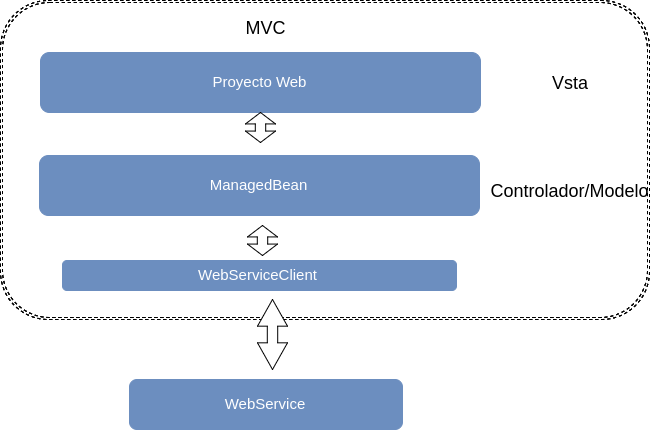
\includegraphics[scale= 0.5]{presentacion}
  \end{center}
  \caption{Separación por capas}
\end{figure}

Como se puede observar en al figura anterior, esta capa está construida por un proyecto Java Server Faces, en el cual, para facilitar el desarrollo y estandarizar el mismo, se utiliza el framework de componentes PrimeFaces.
Dentro de esta capa se crea un proyecto MVC en el cual las páginas xHTML (vistas) se conectan a un ManagedBean (controlador), que a su vez se conecta con una interfaz cliente de los servicios web.

\subsection{Capa de Servicio}

\begin{figure}[H]
  \begin{center}
    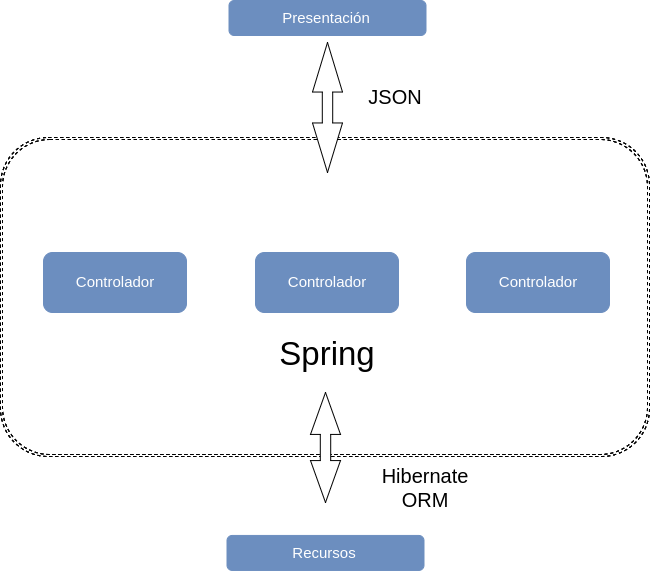
\includegraphics[scale= 0.5]{servicio}
  \end{center}
  \caption{Separación por capas}
\end{figure}

Dentro de esta capa se ejecutan todas las operaciones relacionadas con la lógica de negocio. Estos procesos se representan mediante controladores REST proporcionados por SpringFramework, estos controladores ofrecen una forma sencilla de definir configuraciones a cada endpoint, como ruta del controlador, método HTTP, autenticación, parámetros, entre otros.

Dentro de esta capa también se hace uso de la salida de un ORM, un objeto producto del mapeo objeto-relación. Estos objetos proporcionan una interfaz para manipular realizar operaciones comunes evitando el manejo de sentencias planas SQL.

El modelo SOA tradicionalmente emplea el formato XML para el intercambio de datos entre capa de presentación y de lógica de negocio. En esta propuesta el formato a utilizar será el formato JSON, pues presenta un mejor rendimiento por ser más ligero que XML.

\subsection{Capa de Datos}

\begin{figure}[H]
  \begin{center}
    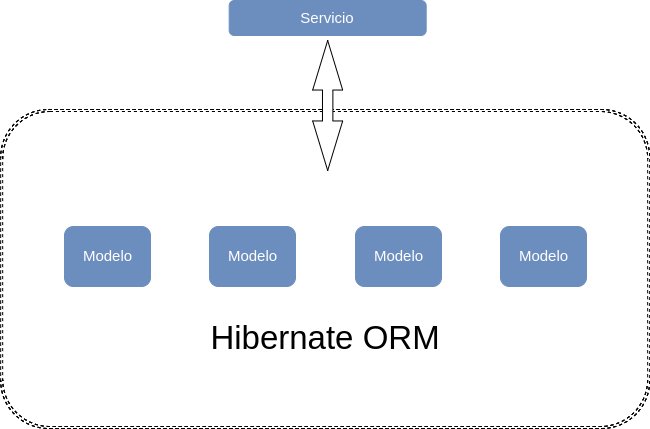
\includegraphics[scale= 0.5]{modelo}
  \end{center}
  \caption{Separación por capas}
\end{figure}

En esta capa se definen los modelos que van a representarán la información necesaria para los procesos que el sistema lleve a cabo.

En esta capa se emplea el framework Hibernate que opera como una capa de abstracción de la Java Persistence API (JPA).

Los modelos antes mencionados permiten una conexión con la Base de Datos que sustituye a las sentencias SQL. 

Al suprimir el uso de SQL se facilita a los desarrolladores objetos con los que están familiarizados, estos objetos incluyen métodos que permiten añadir, modificar, eliminar, etc. registros, aparte de proporcionar la posibilidad de incluir métodos personalizados.
\section{Despliegue}

\begin{figure}[H]
  \begin{center}
    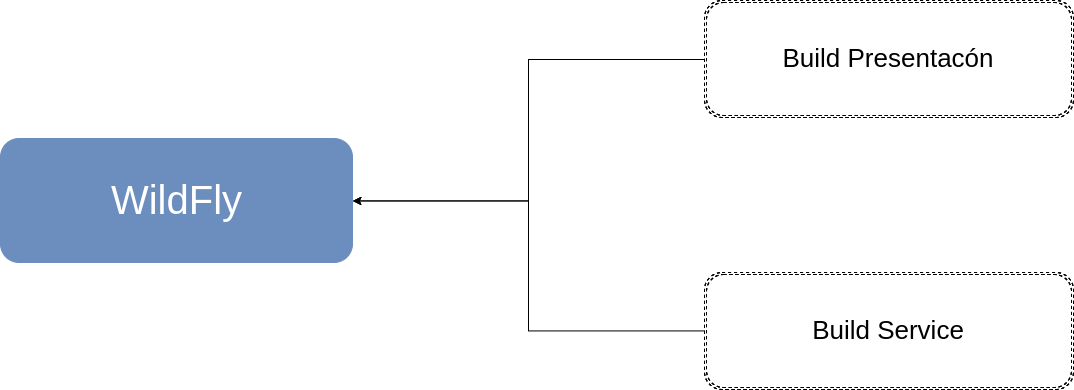
\includegraphics[scale= 0.3]{despliegue}
  \end{center}
  \caption{Separación por capas}
\end{figure}

Una vez que el sistema está construido, se debe llevar a producción. Este proceso se lleva a cabo mediante un despliegue en WildFly.

Para el despliegue se hace un “build” de los proyectos Web y Service, el proyecto model no se compila ya que se usa como “dependencia” del proyecto serivce.

Al terminar el proceso de construcción, se generarán 2 archivos .war, estos archivos serán desplegados al servidor WildFly
\newpage
\section{Diagrama Final de Arquitectura} 

En la siguiente figura se puede observar el diagrama final de los elementos que conforman la propuesta de arquitectura de sistemas de información desarrollados en MBN.

\begin{figure}[H]
  \begin{center}
    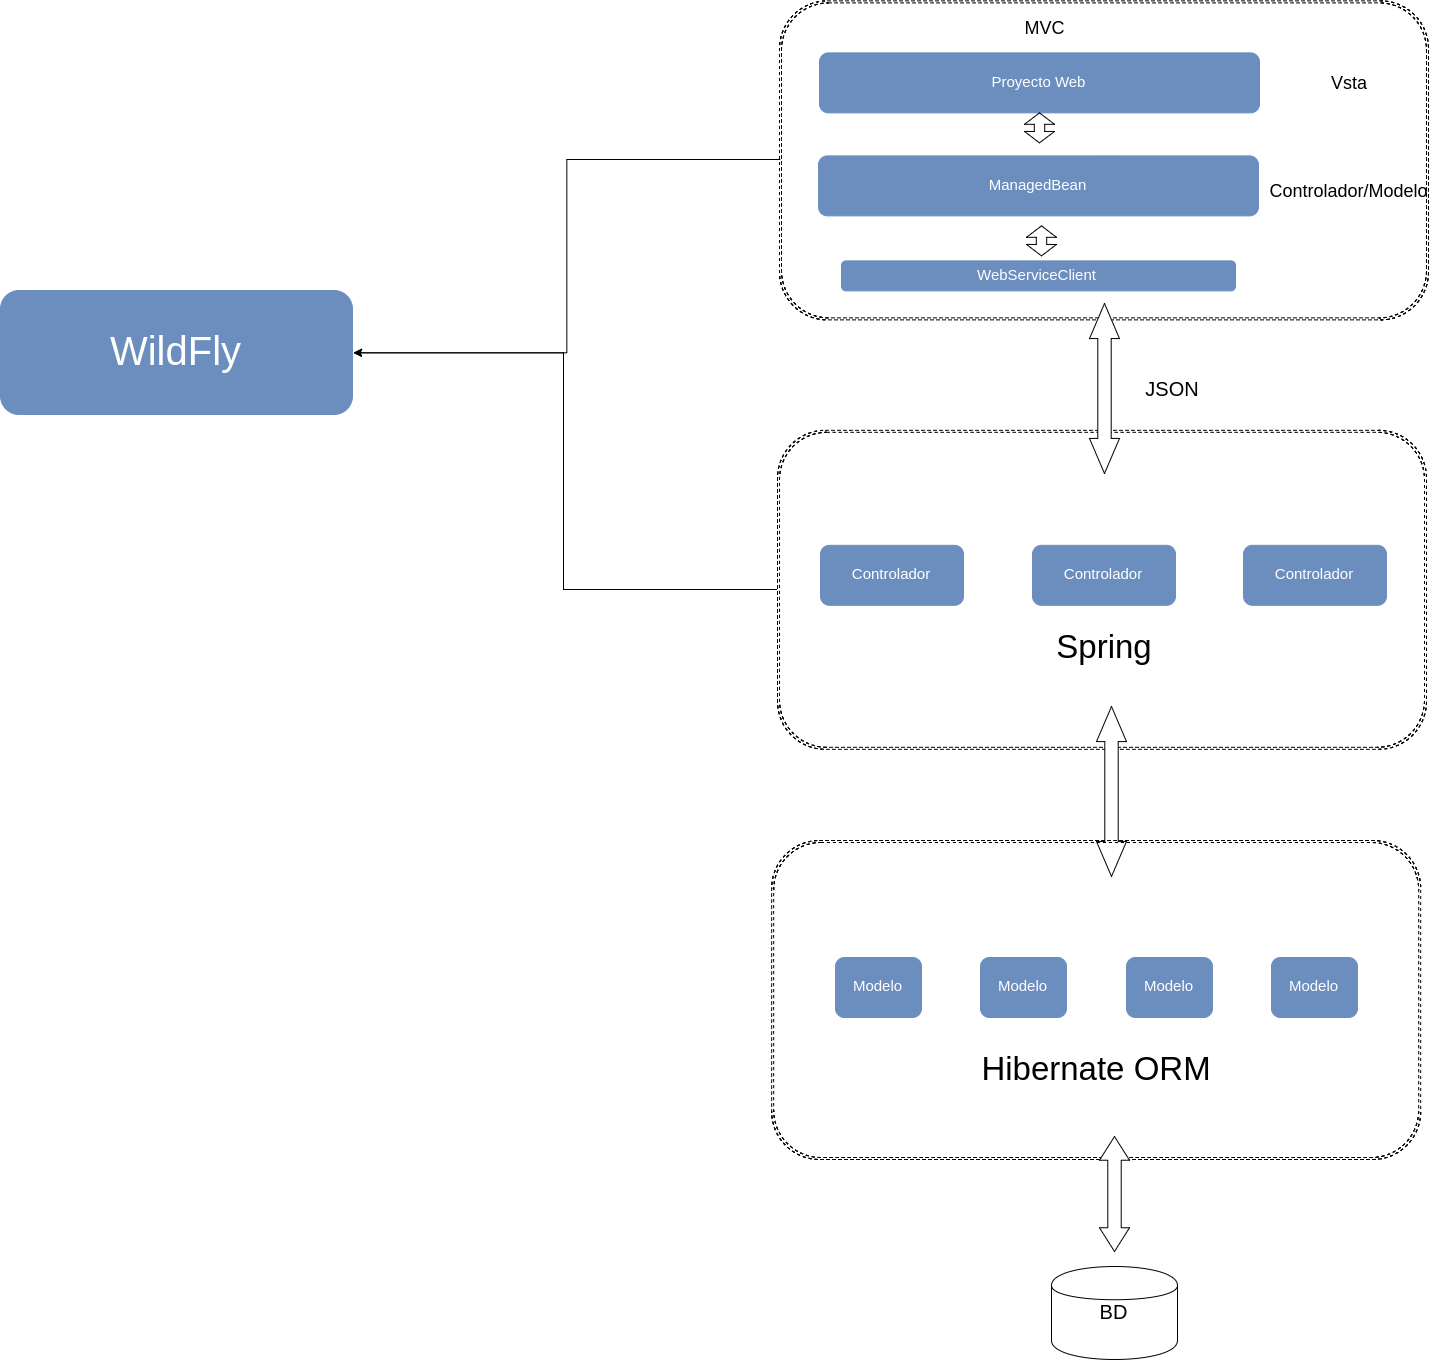
\includegraphics[scale= 0.2]{archcompl}
  \end{center}
  \caption{Separación por capas}
\end{figure}

